\chapter{Despliegue} \label{despliegue}

Con la plataforma ya funcionando en la máquina local es momento de proceder a su despliegue. Actualmente existen múltiples posibilidades para realizar el despliegue de una aplicación web como DigitalOcean, OpenShift, AWS o Microsoft Azure. Tras una comparación de precios se ha elegido \textbf{AWS}, en concreto el servicio \textbf{EC2} que es una máquina virtual que representa un servidor físico, por su barato coste, fiabilidad, seguridad, fácil uso y rapidez para llevar a cabo el despliegue. Para facilitar el despliegue se ha decidido ''dockerizar'' la plataforma con \textbf{Docker} y \textbf{Docker Compose}. Además, se ha utilizado \textbf{Cloudfare} para realizar la compra de un dominio y de \textbf{Let's Encrypt} para la generación gratuita de un certificado SSL diseñado para acelerar la adopción de HTTPS, como bien se indica en el artículo \textit{''Let’s Encrypt: An Automated Certificate
Authority to Encrypt the Entire Web''} \cite{aas2019let}. \bigskip

Así pues, una vez se conocen qué herramientas van a ser utilizadas para llevar a cabo el despliegue, seguidamente se explicará el proceso seguido para ello habiendo investigado previamente cómo llevarlo a cabo a través del libro de Shimon Ifrah \cite{ifrah2019installing}.

\section{Proceso del despliegue}
Primeramente, como se ha comentado en la introducción al capítulo, se ha ''dockerizado'' la plataforma. Para ello se han creado tres archivos: dos \textbf{dockerfiles} para el cliente y para el servidor y un \textbf{docker-compose.yaml} para la orquestación de los dos contenedores docker. Veamos a continuación cada uno por separado:

\begin{itemize}
    \item \textbf{Dockerfile del servidor} (Figura \ref{fig:docker-back}): Se ha elegido la imagen de ''node:18-12-alpine'' ya que la versión 18.12 es la versión LTS de Node.js. Tras especificar dicha versión, se ha establecido el directorio de trabajo en el mostrado en la (Figura \ref{fig:docker-back}) y se ha llevado a cabo la instalación de las dependencias del servidor junto con PM2 para finalmente exponer el contenedor docker en el puerto 8080 y lanzar el servidor.
    
    \begin{figure}[H]
        \centering{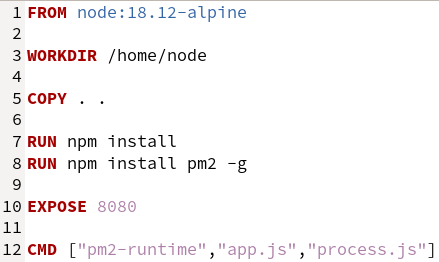
\includegraphics[scale=0.35]{doc/imagenes/docker-back.png
        }}
        \caption{Dockerfile del servidor}
        \label{fig:docker-back}
    \end{figure}
    
    \item \textbf{Dockerfile del cliente} (Figura \ref{fig:docker-front}): El dockerfile del cliente se ha planteado de igual forma al del servidor, con una pequeña diferencia. Se trata de la instalación de las dependencias instaladas en la aplicación de Angular que se encuentran alojadas en el fichero ''package.json''. En cuanto al puerto, se ha elegido el 4200 ya que la aplicaciones de Angular típicamente son expuestas en este puerto.
    
    \begin{figure}[H]
        \centering{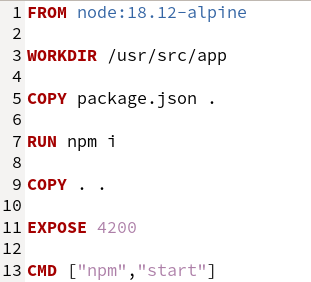
\includegraphics[scale=0.35]{doc/imagenes/docker-front.png}}
        \caption{Dockerfile del cliente}
        \label{fig:docker-front}
    \end{figure}

    \item\textbf{Fichero Docker Compose} (Figura \ref{fig:docker-compose}): Para el fichero '''docker-compose.yaml''' se han establecido dos servicios, uno para el cliente y otro para el servidor. Se han mantenido ambos puertos para la máquina local, pero cuando se haga el despliegue el puerto del cliente, que es el que quedará abierto para acceder a la página, será cambiado de 4200 a 443 que es el puerto usado por HTTPS.

    \begin{figure}[H]
        \centering{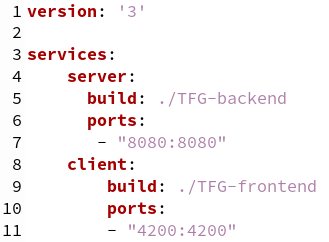
\includegraphics[scale=0.35]{doc/imagenes/docker-compose.png}}
        \caption{Fichero Docker Compose}
        \label{fig:docker-compose}
    \end{figure}
\end{itemize}


Ahora que el proyecto ha sido dockerizado y con una cuenta ya creada en AWS, se lanza la instancia EC2. Esta tarea resulta algo compleja, ya que implica hacer un pequeño estudio del consumo de memoria y CPU de los contenedores docker para su configuración. Gracias a la orden '''docker stats''' podemos visualizar dichas métricas (Figura \ref{fig:docker-stats}):

    \begin{figure}[H]
        \centering{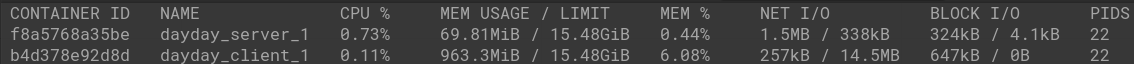
\includegraphics[scale=0.35]{doc/imagenes/docker-stats.png}}
        \caption{Consumo de los contenedores docker del servidor y del cliente}
        \label{fig:docker-stats}
    \end{figure}

Teniendo estas métricas presentes, la configuración escogida para la instancia ha sido la siguiente:
\begin{itemize}
    \item \textbf{Sistema operativo}: Debido a que
    a que pertenece al plan gratuito, se ha escogido la imagen del sistema operativo Linux de Amazon con la arquitectura presentada en la Figura \ref{fig:ec2-imagen}:
    \begin{figure}[H]
        \centering{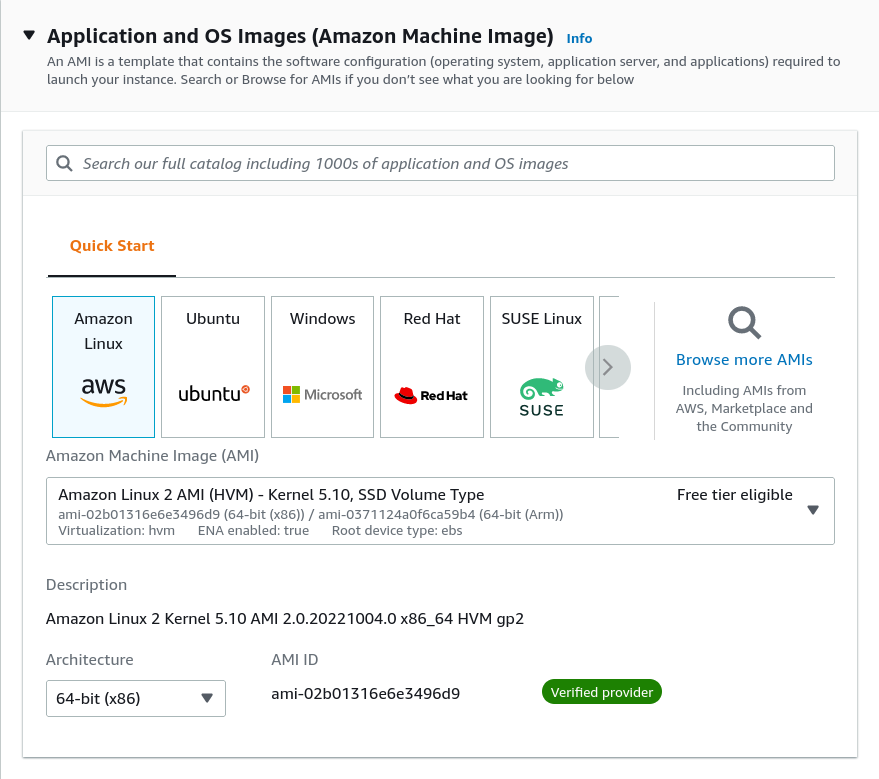
\includegraphics[scale=0.25]{doc/imagenes/imagen-aws.png}}
        \caption{Imagen escogida para la instancia de EC2}
        \label{fig:ec2-imagen}
    \end{figure}
    \item \textbf{Tipo de instancia}: Son numerosas los tipos de instancias ofrecidas para EC2, pero visualizando la Figura \ref{fig:docker-stats} donde se aprecia un consumo de ran de casi 1GiB por parte del contenedor del cliente y entorno a 80MiB por parte del servidor, se ha barajado entre escoger una instancia ''t2.small'' o ''t3.medium'' (Figura \ref{fig:ec2-types}). Finalmente, se ha optado por la segunda opción con el objetivo de evitar limitaciones de RAM:
    \begin{figure}[H]
        \centering{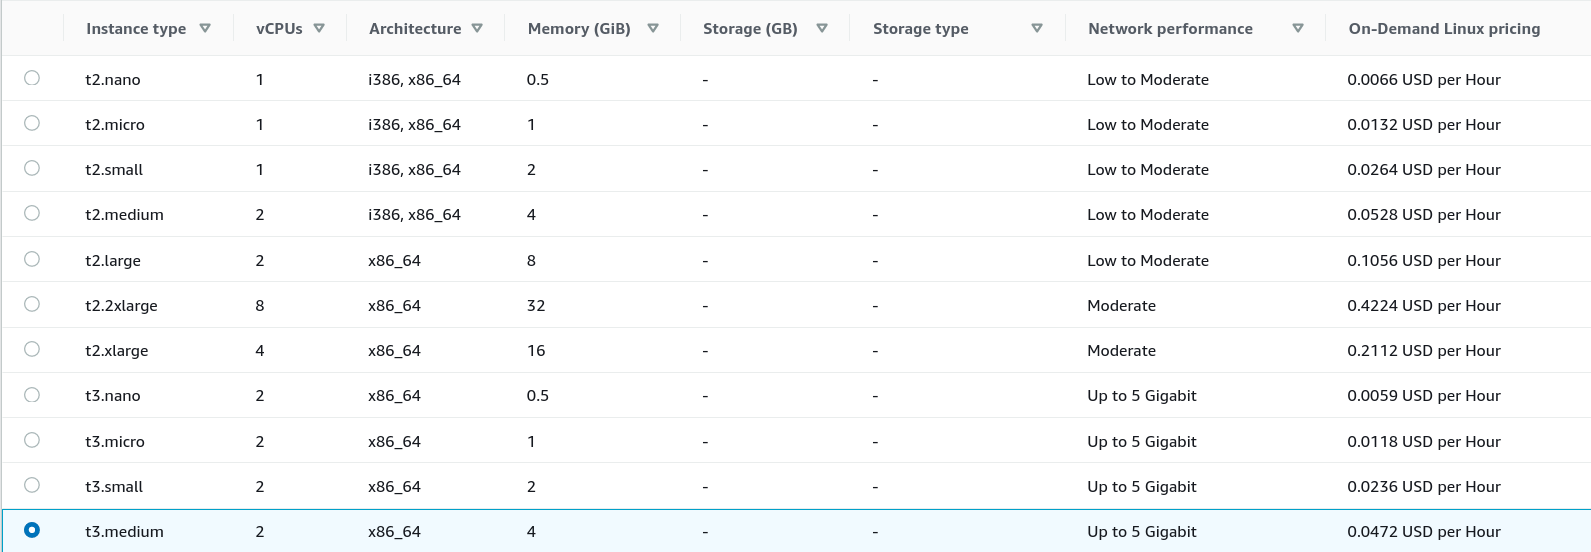
\includegraphics[scale=0.25]{doc/imagenes/aws-type.png}}
        \caption{Tipos de instancias EC2 junto con sus características y precios}
        \label{fig:ec2-types}
    \end{figure}
    \item \textbf{Grupos de seguridad}: Finalmente se han establecido los grupos de seguridad, que funcionan a modo de firewall dictando quin puede entrar a la instancia. En este caso se han establecido tres: SSH, HTTP y HTTPS, a través de los cuales todo el mundo pueda acceder a la plataforma (Figura \ref{fig:ec2-security}):
    \begin{figure}[H]
        \centering{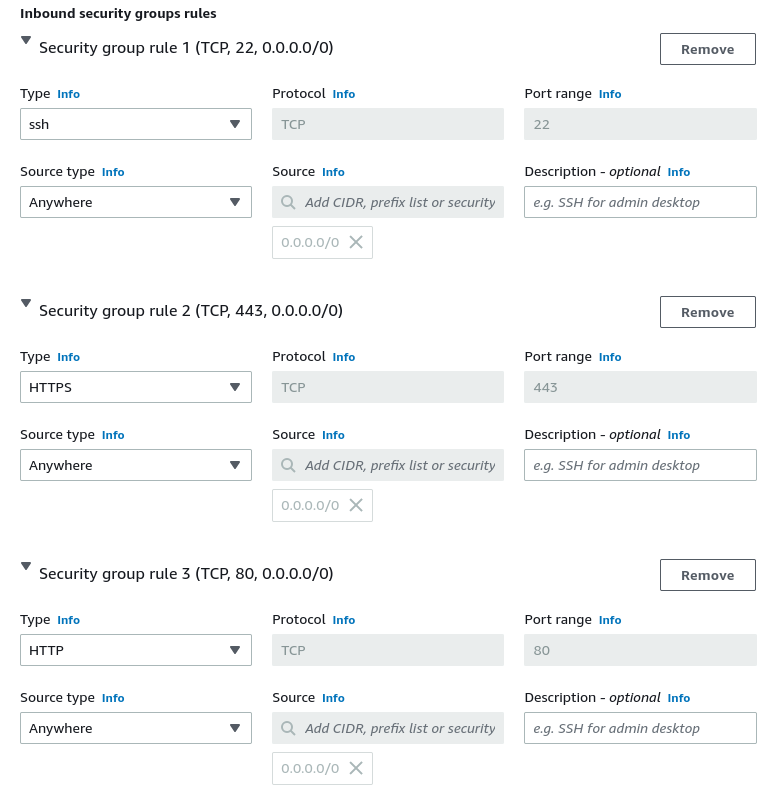
\includegraphics[scale=0.25]{doc/imagenes/aws-security.png}}
        \caption{Grupos de seguridad establecidos para la instancia EC2}
        \label{fig:ec2-security}
    \end{figure}
\end{itemize}

Con esta configuración lista ya se puede lanzar la instancia y hacer la conexión vía ssh a ella. Una vez se ha realizado la conexión se procede a descargar el repositorio de Github de este proyecto y se lanza la orden '''docker-compose up'''.  \bigskip

Por último, se ha hecho la compra del dominio ''dayday-calendar.win'' en Cloudfare. Se ha escogido este dominio en específico debido a ser el que más bajo coste tenía y se le han asignado la IPs pública de la instancia EC2 (Figura \ref{fig:dns})

    \begin{figure}[H]
        \centering{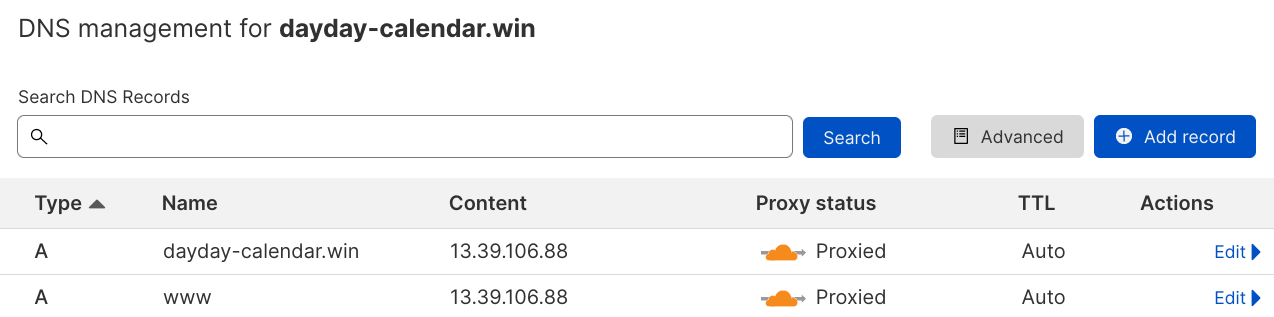
\includegraphics[scale=0.25]{doc/imagenes/dns.png}}
        \caption{Asignación de la IP pública de la instancia EC2 al dominio}
        \label{fig:dns}
    \end{figure}

Para acabar, creamos una zona alojada con el servicio ''Route 53'' de AWS para el dominio de Cloudfare. Esto es necesario para gestionar la dirección del tráfico hacia un dominio en específico (Figura \ref{fig:aws-zone}):

    \begin{figure}[H]
        \centering{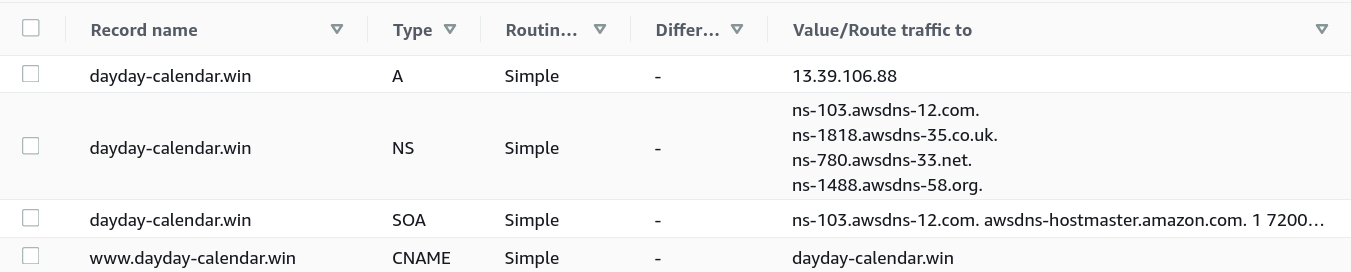
\includegraphics[scale=0.25]{doc/imagenes/aws-zone.png}}
        \caption{Zonas alojadas para la instancia}
        \label{fig:aws-zone}
    \end{figure}

En cuanto a la generación del certificado se ha hecho uso de las indicaciones dadas por la página oficial de Let's Encrypt donde indican que a través de la ejecución del cliente \textbf{Certbot} ,que deberá previamente ser instalado en la instancia, y se crearán el archivo del certificado y la llave de éste. 